\chapter{Лекция 8. Алгоритм Краскала. Главные циклы. Цикловое пространство}

% ============================================================
% АЛГОРИТМ КРАСКАЛА
% ============================================================

$G(V, E)$ --- связный, $\sigma\colon E \to \mathbb{R}$.

$\Rightarrow\; T_G(V, \hat{E})$ --- остовное дерево ($\min \sum \sigma(e),\; e \in \hat{E}$).

\begin{algo}{Алгоритм Краскала}{kruskal}

\textbf{Step:} рёбра перебираются в порядке возрастания веса; очередное
ребро $e$ с минимальным $\sigma(e)$ добавляется в остов, если при этом
\emph{не появляется цикл} (т.\,е. концы $e$ лежат в разных компонентах
уже построенного леса); иначе ребро пропускается.

\medskip
\noindent\textbf{Пример} (граф той же структуры, что у алгоритма Прима,
с другими весами):

% Граф: p20-kraskal-example-1.graph
\grfig[0.55]{figures/p20-kraskal-example-1.pdf}{Алг. Краскала: взвешенный граф 9 вершин}

\medskip
\begin{center}
\begin{tabular}{c|c|c|l}
$V$ & $e$ & $\sum \sigma(e)$ & комментарий \\ \hline
---     & ---      & 0  & лес из 9 изолированных вершин \\
$J, I$  & $JI(1)$  & 1  & соединяем $\{J\}$ и $\{I\}$ \\
$B, C$  & $BC(2)$  & 3  & соединяем $\{B\}$ и $\{C\}$ \\
$A, D$  & $AD(3)$  & 6  & соединяем $\{A\}$ и $\{D\}$ \\
$H$     & $HD(4)$  & 10 & $H$ присоединяется к $\{A, D\}$ \\
$F$     & $AF(5)$  & 15 & $F$ присоединяется к $\{A, D, H\}$ \\
$E$     & $DE(6)$  & 21 & $E$ присоединяется к $\{A, D, H, F\}$ \\
---     & $JD(7)$  & 28 & сливаем $\{J, I\}$ и $\{A, D, H, F, E\}$ \\
---     & $BD(8)$  & 36 & сливаем $\{B, C\}$ с остальными; $8$ рёбер --- стоп \\
\end{tabular}
\end{center}

\medskip
Оставшиеся рёбра $EC(9)$, $BE(10)$, $AB(11)$, $FH(12)$, $HI(13)$,
$EJ(14)$ замыкали бы циклы и пропускаются. Минимальное остовное дерево:
$JI, BC, AD, HD, AF, DE, JD, BD$, суммарный вес $\sum\sigma = 36$.

\medskip
\textbf{Упр.} Почему алгоритм сойдётся (построит остов)?

\textit{Ответ.} Каждое добавленное ребро уменьшает число компонент леса
ровно на $1$: начали с $|V|$ компонент, дерево получится после $|V| - 1$
добавлений. Застрять алгоритм не может: пока компонент больше одной,
в связном графе обязательно найдётся ребро между разными компонентами
--- и при просмотре списка оно не будет пропущено.

\medskip
\noindent\textbf{Работа алгоритма по шагам} (добавленные рёбра ---
зелёные, текущее --- оранжевое, пропущенные --- бледно-серые):

\begin{center}\begin{tabular}{ccc}
\shortstack{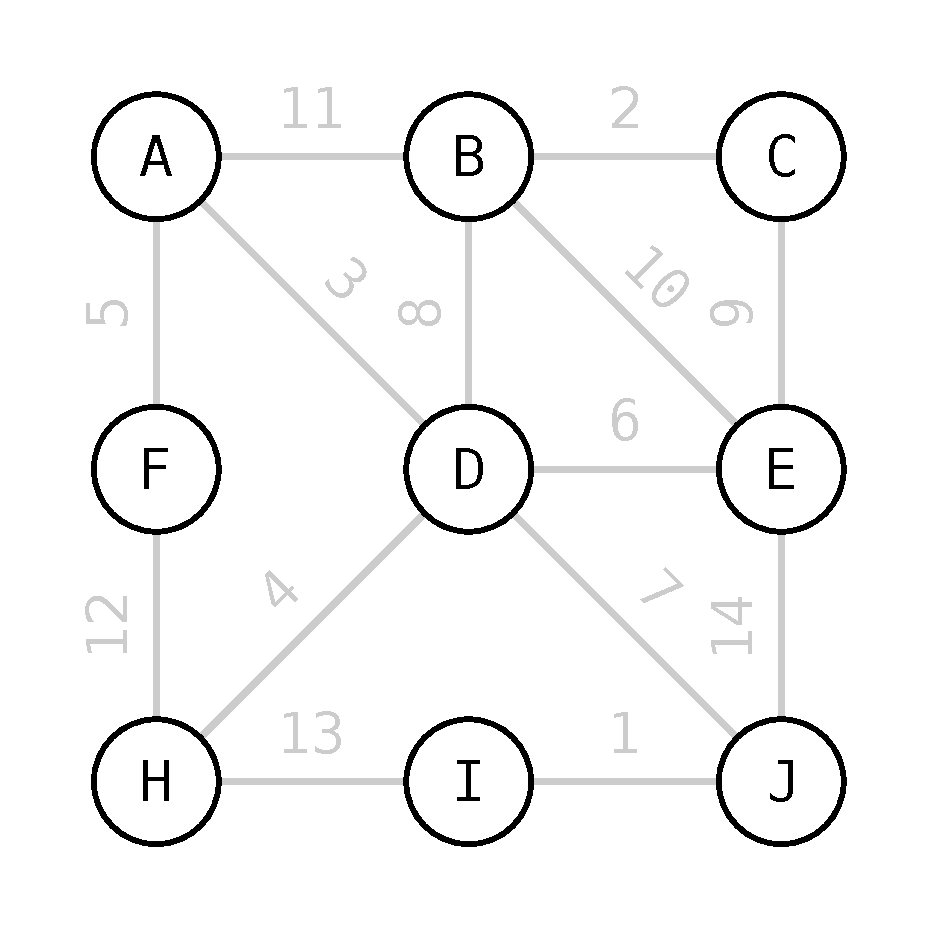
\includegraphics[width=0.30\textwidth]{python/lec08/kruskal/kruskal-0.pdf}\\[2pt]{\scriptsize Шаг 0. Лес из изолированных вершин}} &
\shortstack{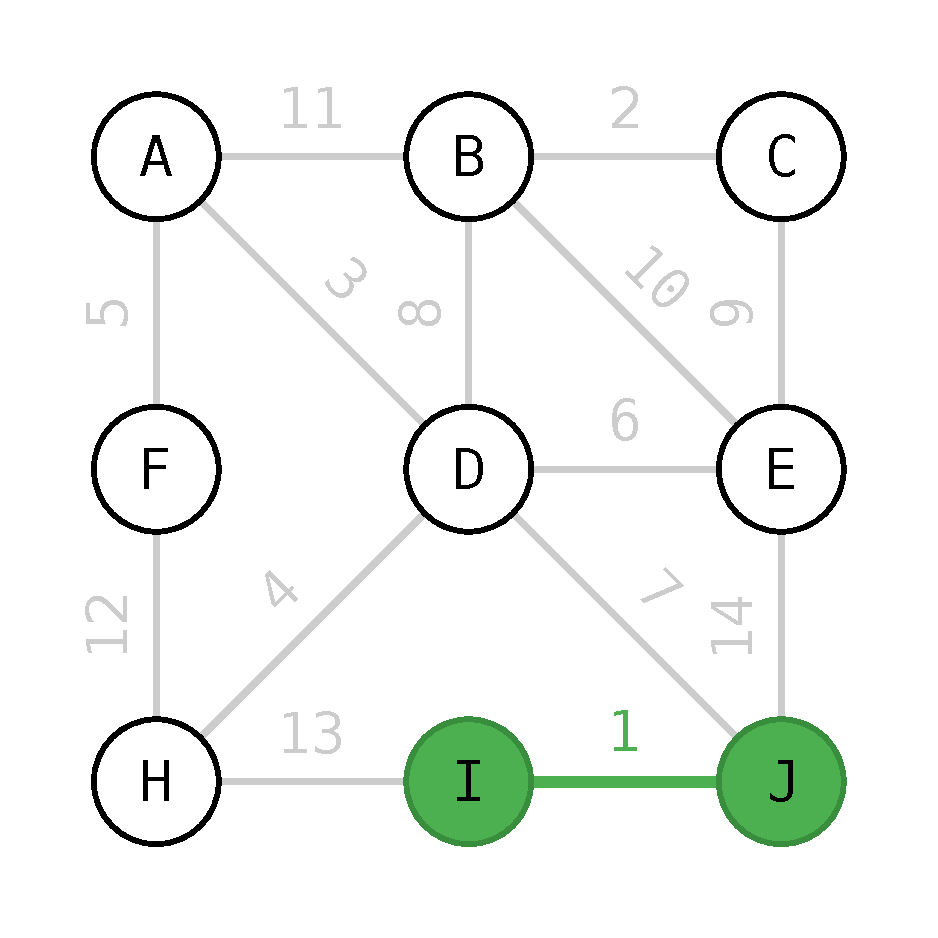
\includegraphics[width=0.30\textwidth]{python/lec08/kruskal/kruskal-1.pdf}\\[2pt]{\scriptsize Шаг 1. $+JI(1)$}} &
\shortstack{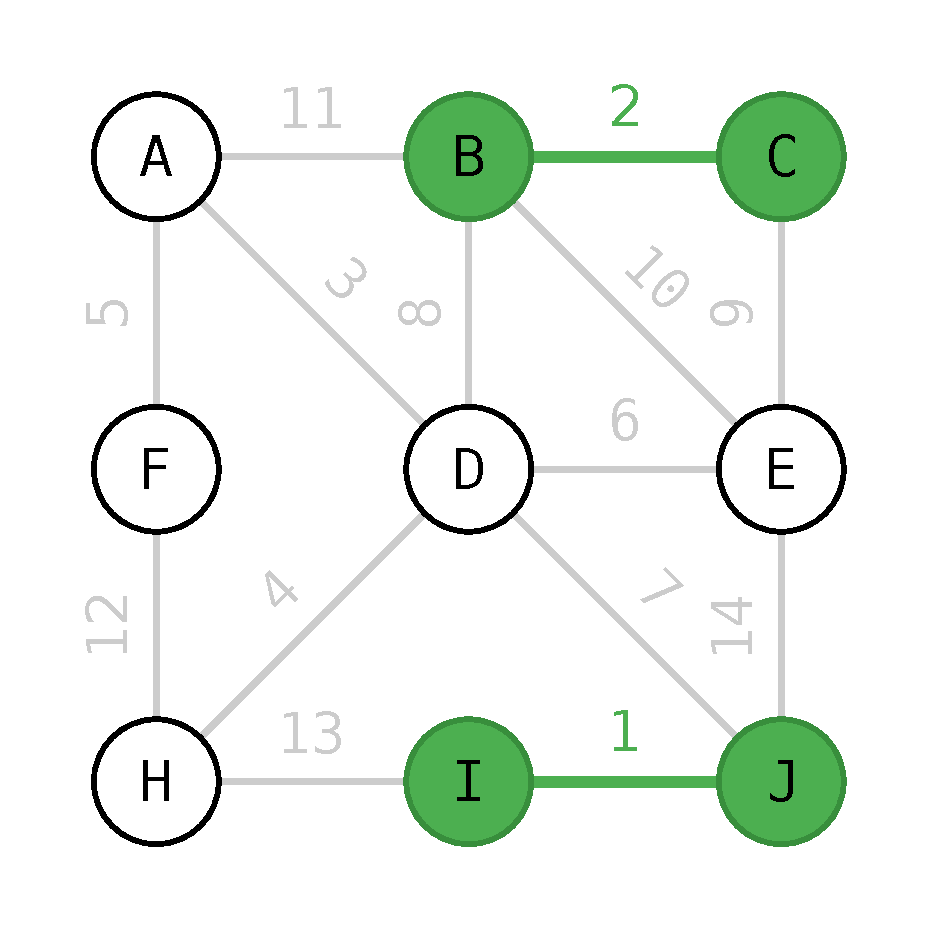
\includegraphics[width=0.30\textwidth]{python/lec08/kruskal/kruskal-2.pdf}\\[2pt]{\scriptsize Шаг 2. $+BC(2)$}} \\
\end{tabular}\end{center}
\begin{center}\begin{tabular}{ccc}
\shortstack{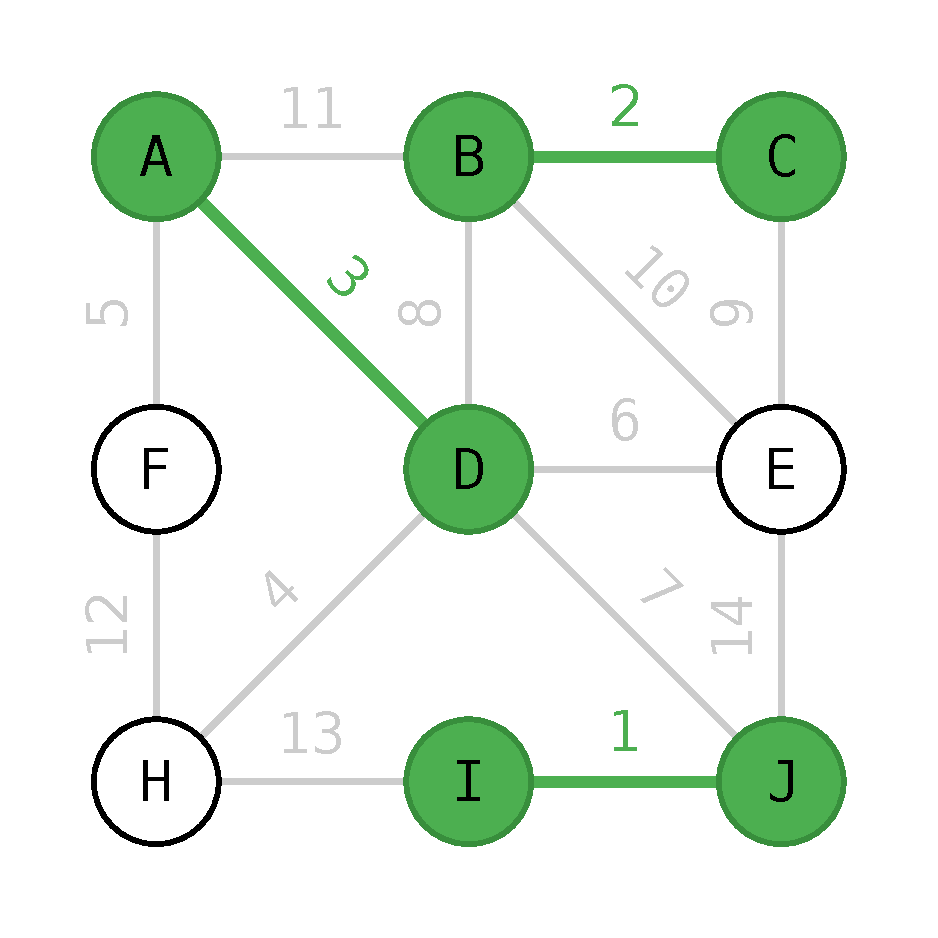
\includegraphics[width=0.30\textwidth]{python/lec08/kruskal/kruskal-3.pdf}\\[2pt]{\scriptsize Шаг 3. $+AD(3)$}} &
\shortstack{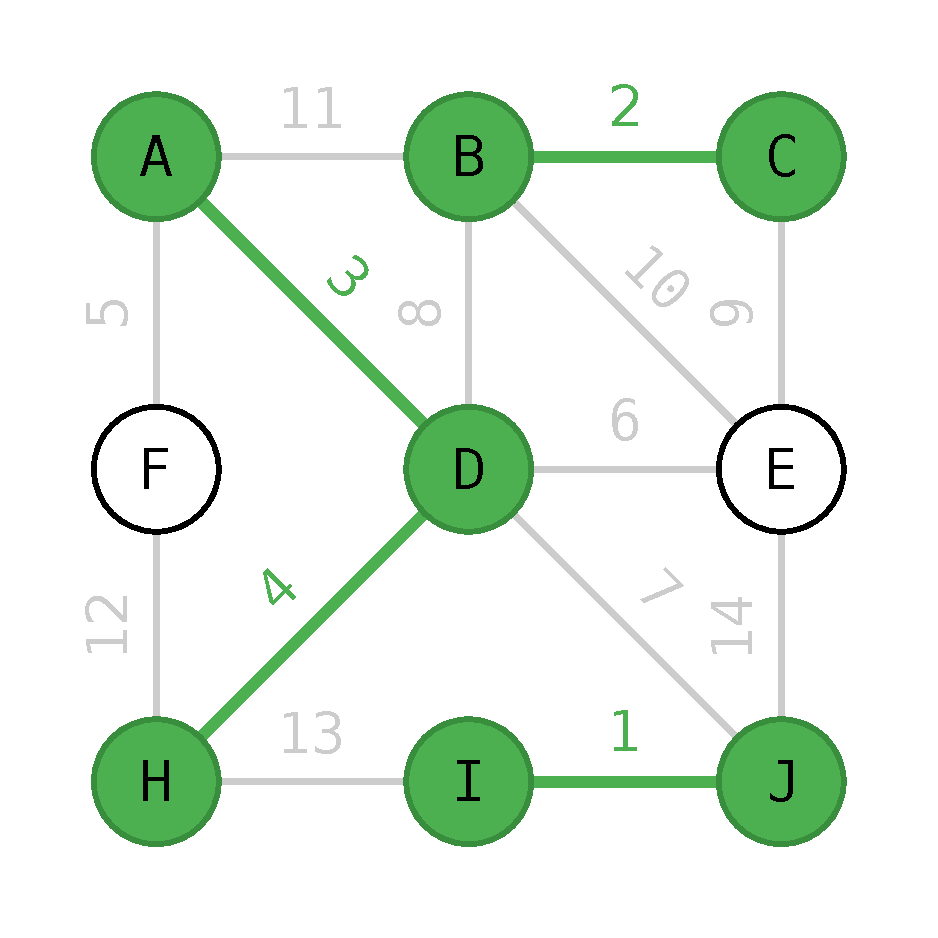
\includegraphics[width=0.30\textwidth]{python/lec08/kruskal/kruskal-4.pdf}\\[2pt]{\scriptsize Шаг 4. $+HD(4)$}} &
\shortstack{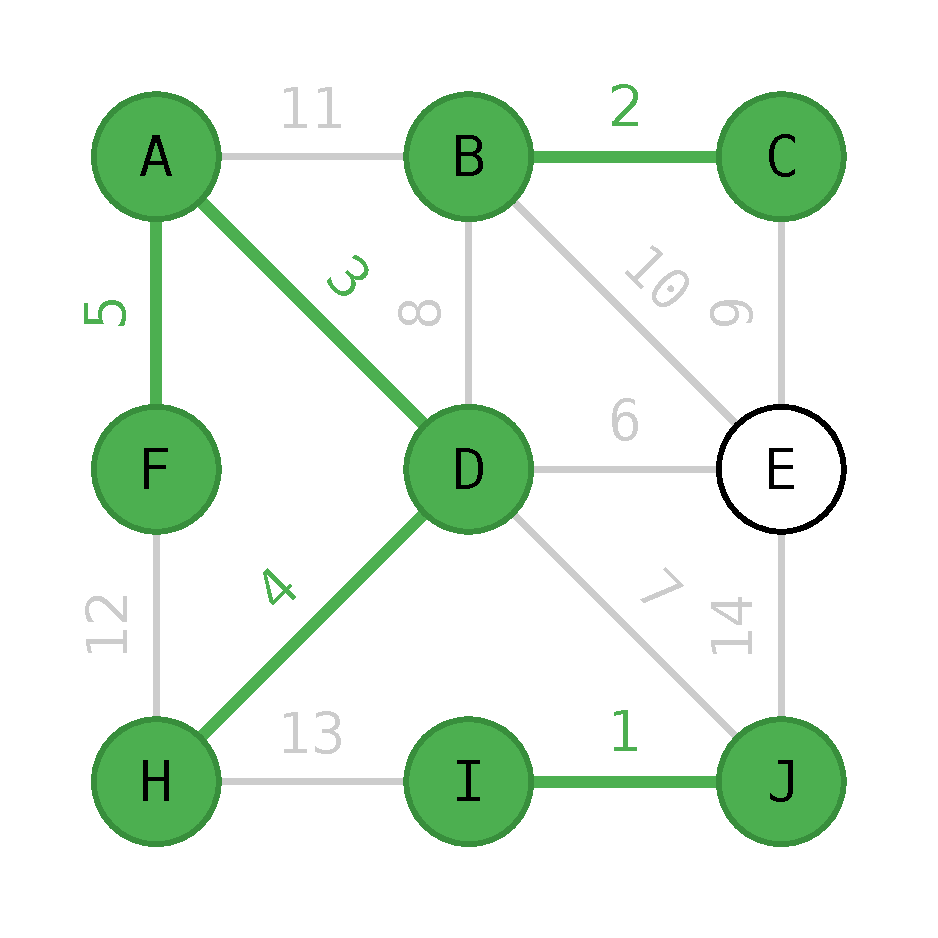
\includegraphics[width=0.30\textwidth]{python/lec08/kruskal/kruskal-5.pdf}\\[2pt]{\scriptsize Шаг 5. $+AF(5)$}} \\
\end{tabular}\end{center}
\begin{center}\begin{tabular}{ccc}
\shortstack{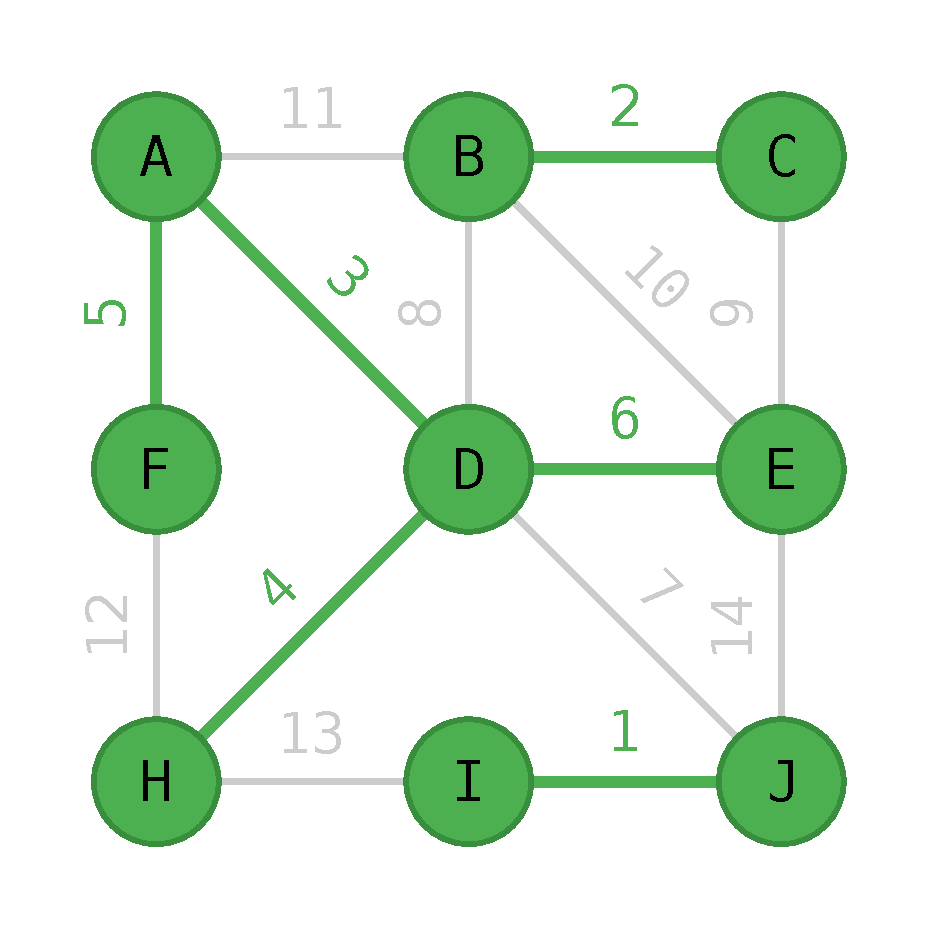
\includegraphics[width=0.30\textwidth]{python/lec08/kruskal/kruskal-6.pdf}\\[2pt]{\scriptsize Шаг 6. $+DE(6)$}} &
\shortstack{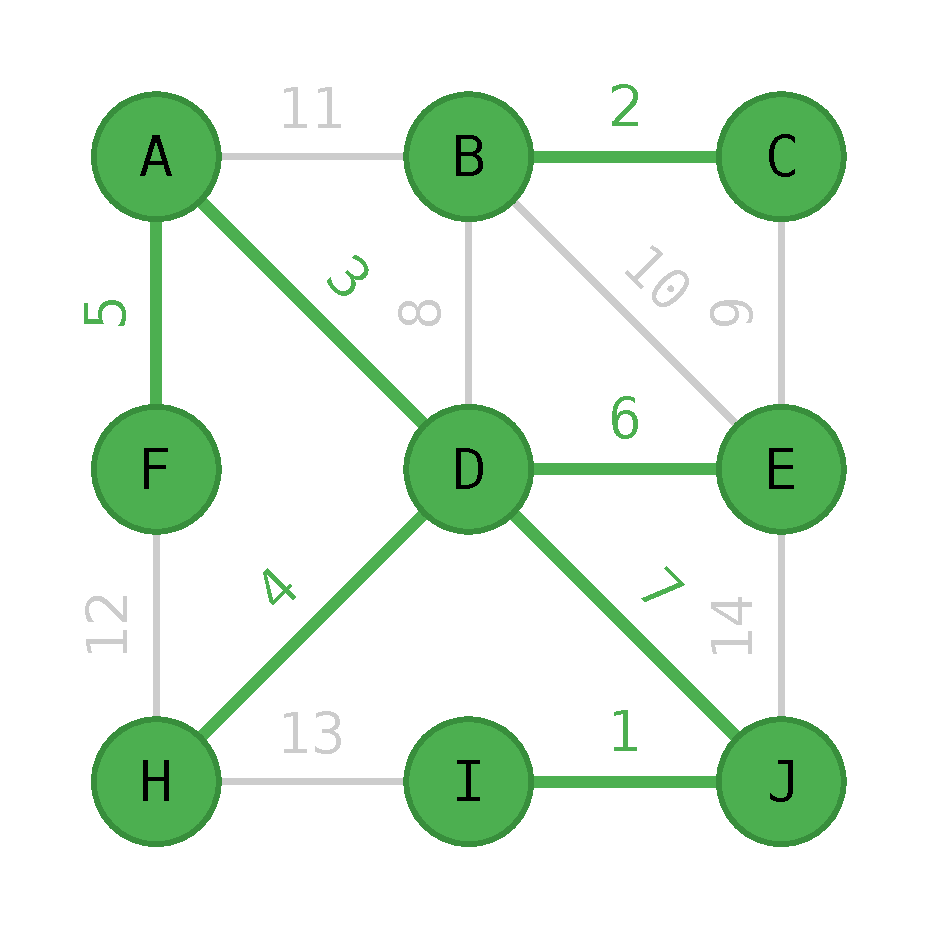
\includegraphics[width=0.30\textwidth]{python/lec08/kruskal/kruskal-7.pdf}\\[2pt]{\scriptsize Шаг 7. $+JD(7)$}} &
\shortstack{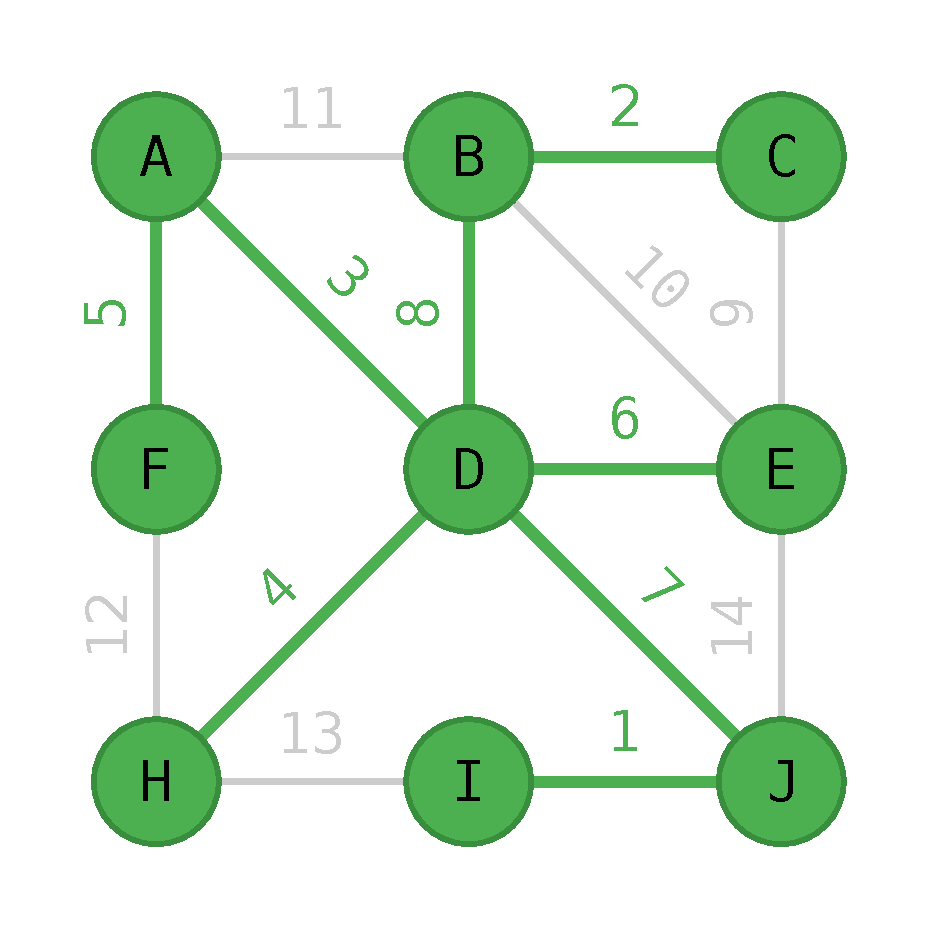
\includegraphics[width=0.30\textwidth]{python/lec08/kruskal/kruskal-8.pdf}\\[2pt]{\scriptsize Шаг 8. $+BD(8)$: остов готов}} \\
\end{tabular}\end{center}
\begin{center}\begin{tabular}{ccc}
\shortstack{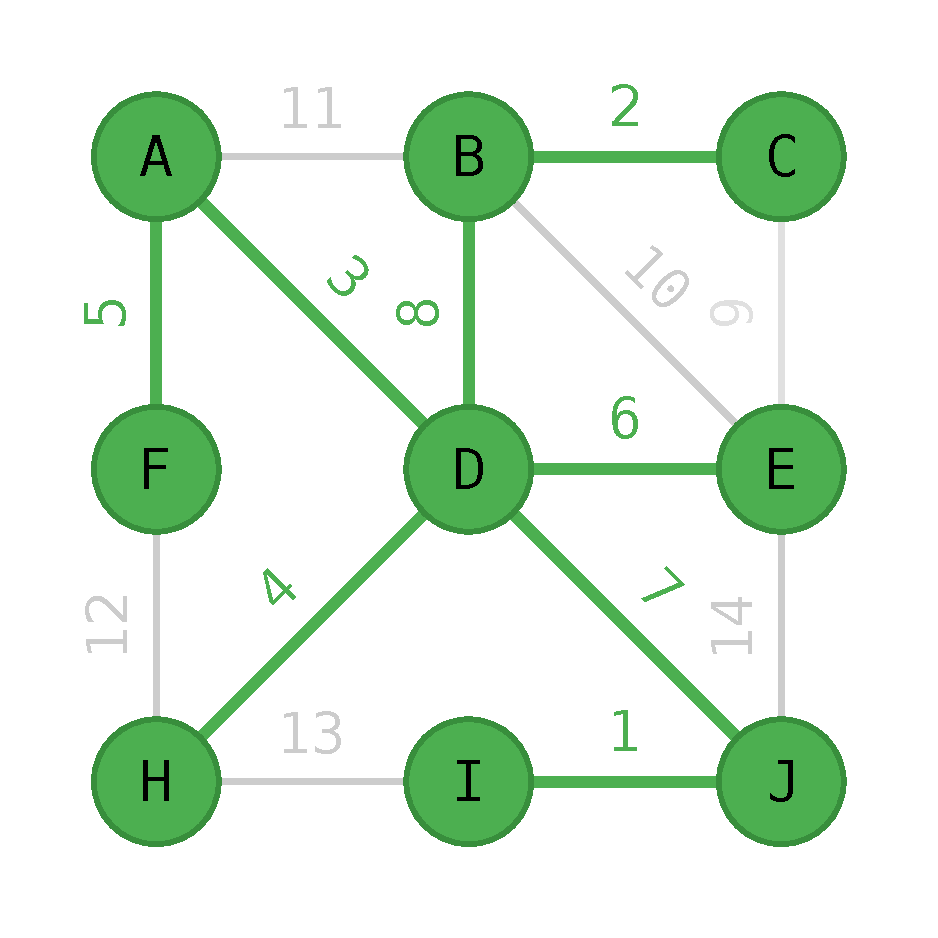
\includegraphics[width=0.30\textwidth]{python/lec08/kruskal/kruskal-9.pdf}\\[2pt]{\scriptsize Шаг 9. $EC(9)$ --- цикл, пропуск}} &
\shortstack{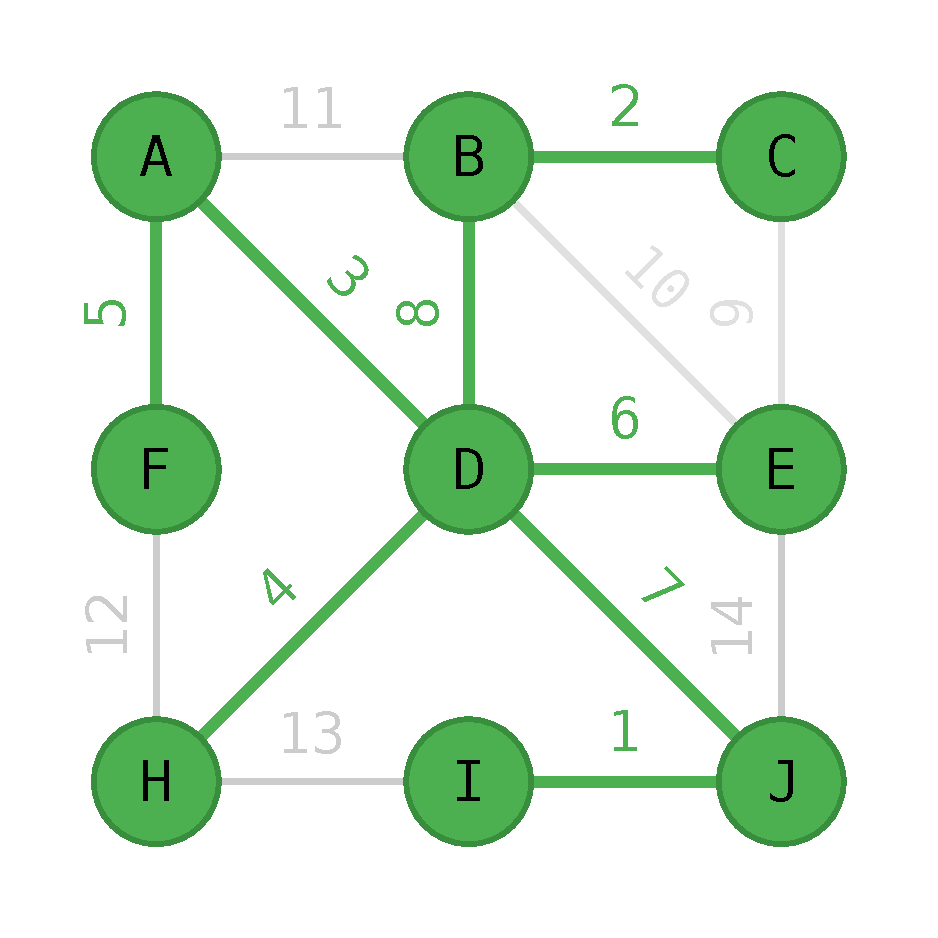
\includegraphics[width=0.30\textwidth]{python/lec08/kruskal/kruskal-10.pdf}\\[2pt]{\scriptsize Шаг 10. $BE(10)$ --- пропуск}} &
\shortstack{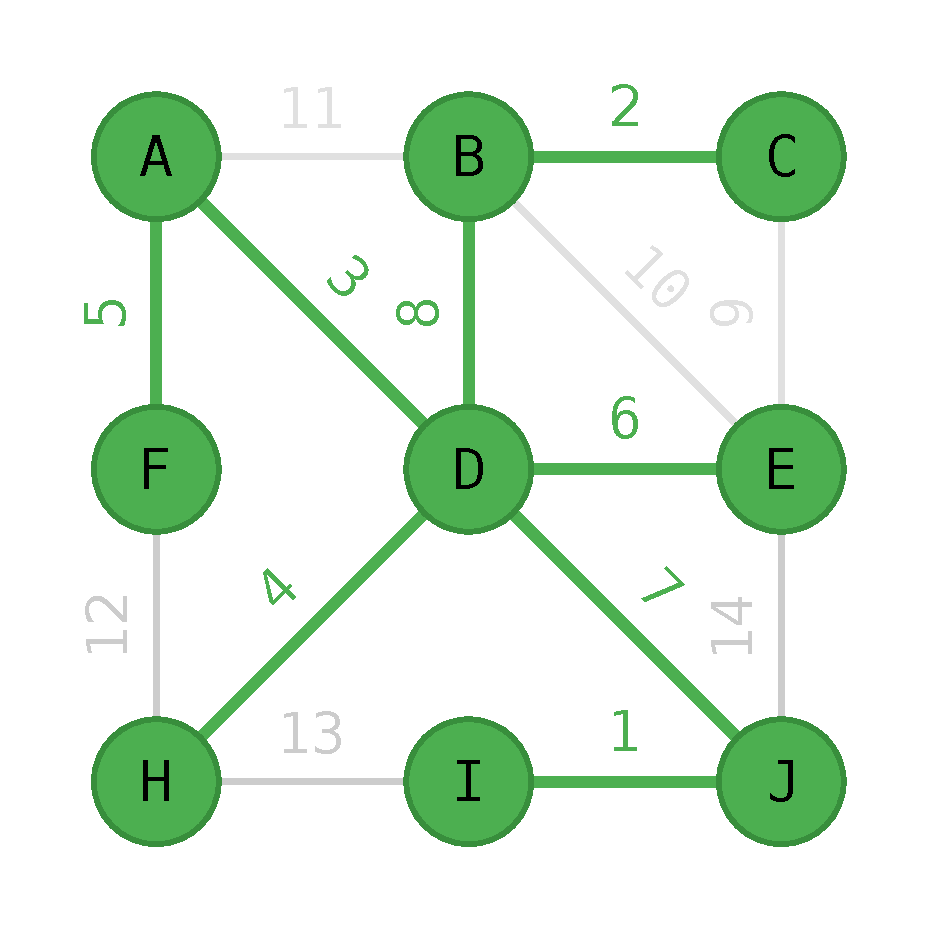
\includegraphics[width=0.30\textwidth]{python/lec08/kruskal/kruskal-11.pdf}\\[2pt]{\scriptsize Шаг 11. $AB(11)$ --- пропуск}} \\
\end{tabular}\end{center}
\begin{center}\begin{tabular}{ccc}
\shortstack{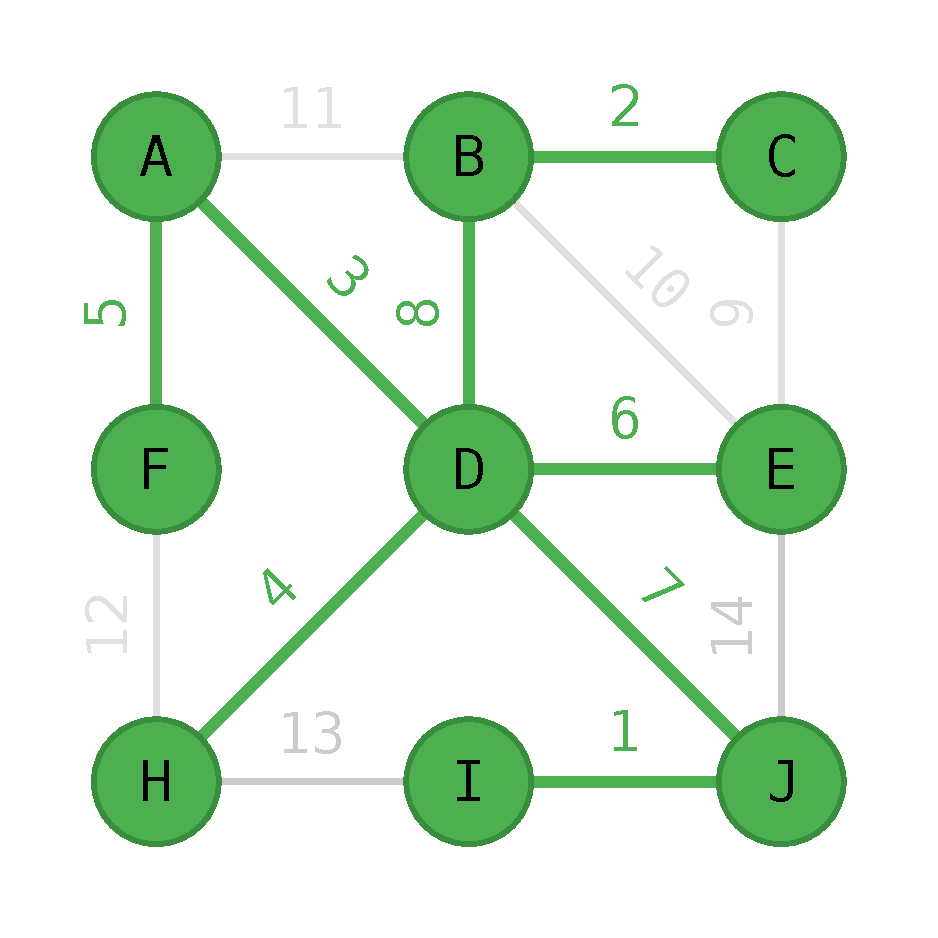
\includegraphics[width=0.30\textwidth]{python/lec08/kruskal/kruskal-12.pdf}\\[2pt]{\scriptsize Шаг 12. $FH(12)$ --- пропуск}} &
\shortstack{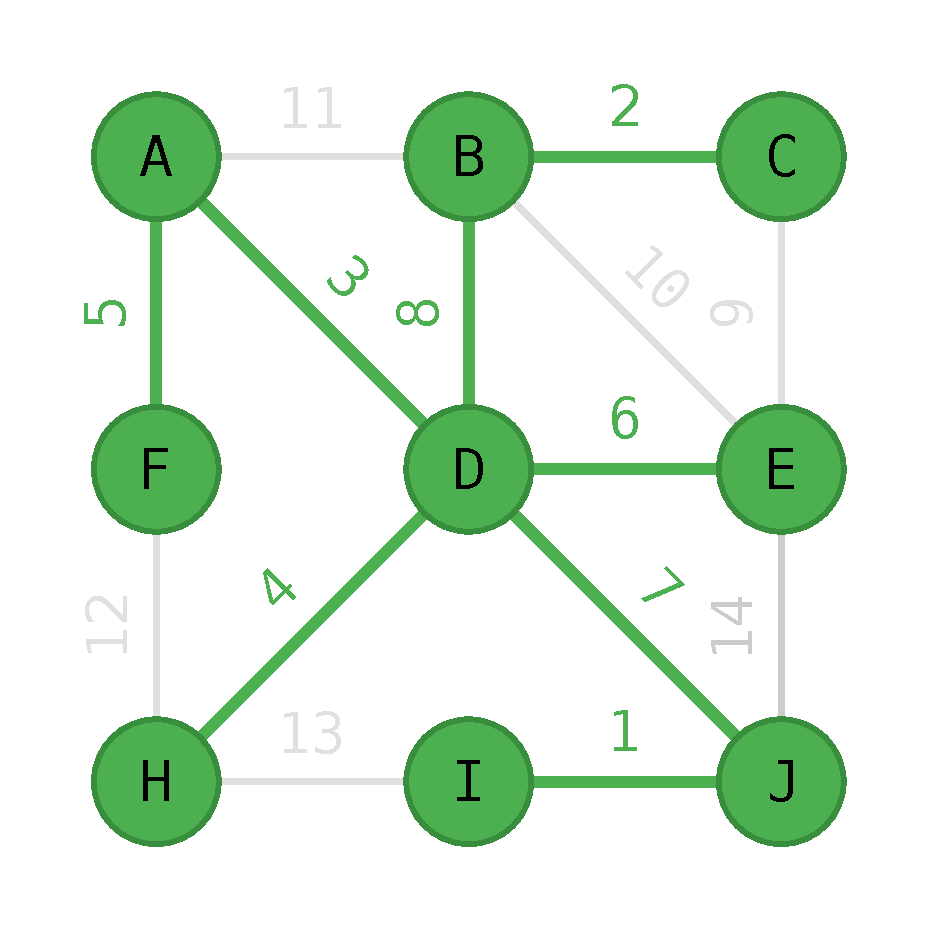
\includegraphics[width=0.30\textwidth]{python/lec08/kruskal/kruskal-13.pdf}\\[2pt]{\scriptsize Шаг 13. $HI(13)$ --- пропуск}} &
\shortstack{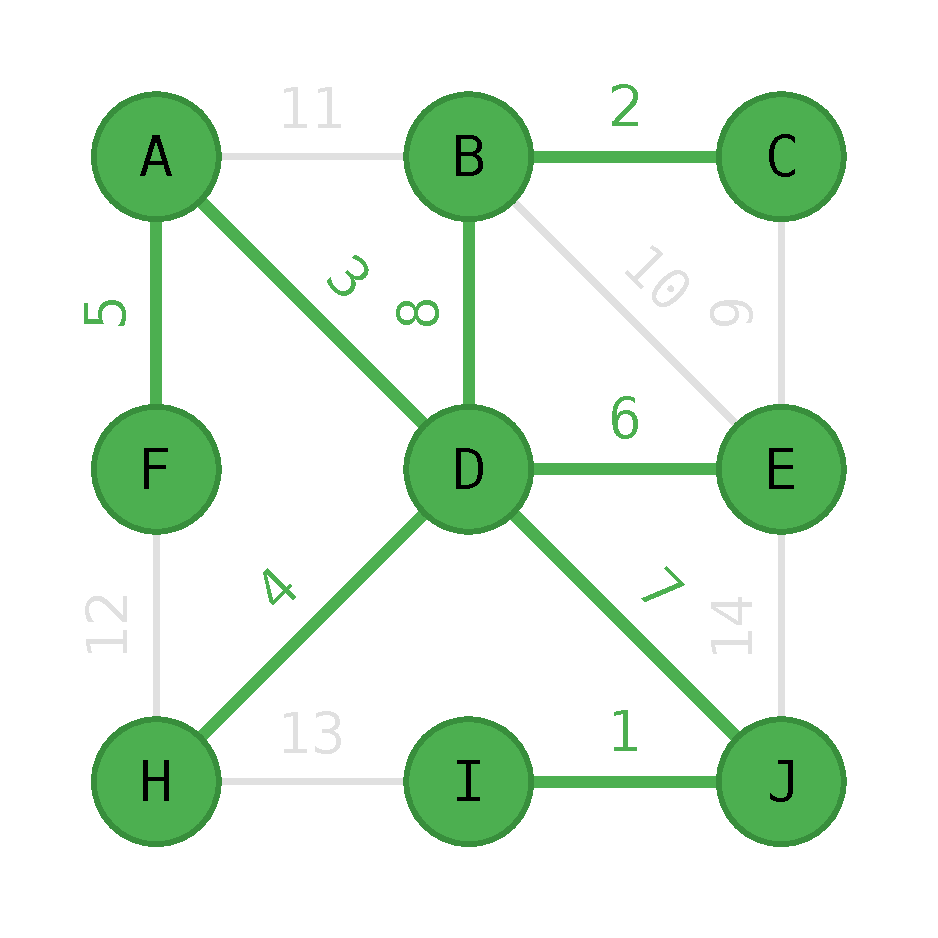
\includegraphics[width=0.30\textwidth]{python/lec08/kruskal/kruskal-14.pdf}\\[2pt]{\scriptsize Шаг 14. $EJ(14)$ --- пропуск}} \\
\end{tabular}\end{center}
\begin{center}
\shortstack{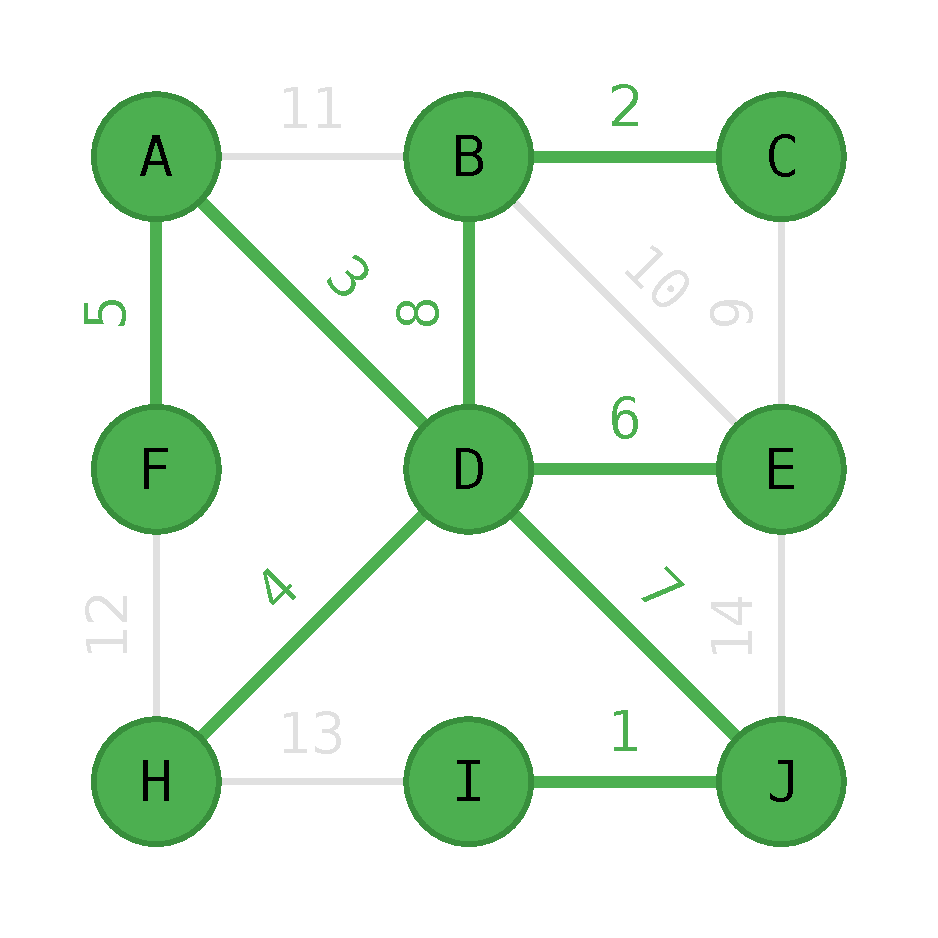
\includegraphics[width=0.32\textwidth]{python/lec08/kruskal/kruskal-15.pdf}\\[2pt]{\scriptsize Шаг 15. Остов построен, $\Sigma = 36$}}
\end{center}
\end{algo}

% ============================================================
% ГЛАВНЫЕ ЦИКЛЫ
% ============================================================

\subsection*{Главные циклы}

\begin{defn}{Хорда}{chord}
$G(V, E)$ --- связный, невзвешенный.

$T_G(V, \hat{E})$ --- остовное дерево $G$.

\textbf{Хорда} $\;\leftrightarrow\;$ $e \in (E \setminus \hat{E})$.
\end{defn}

Зафиксируем в графе остовное дерево; все рёбра вне остова --- хорды:

\begin{center}\begin{tabular}{cc}
\shortstack{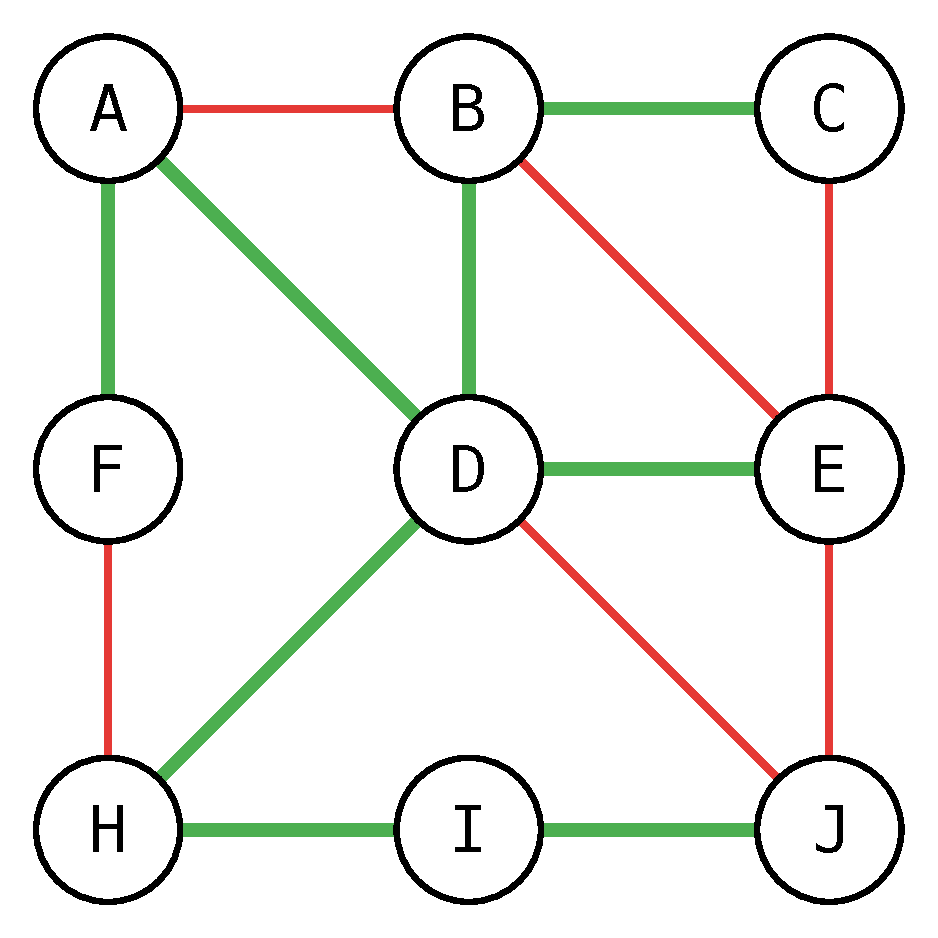
\includegraphics[width=0.42\textwidth]{figures/p20-chords-graph.pdf}\\[2pt]{\scriptsize а) граф $G$: остов --- зелёным, хорды --- красным}} &
\shortstack{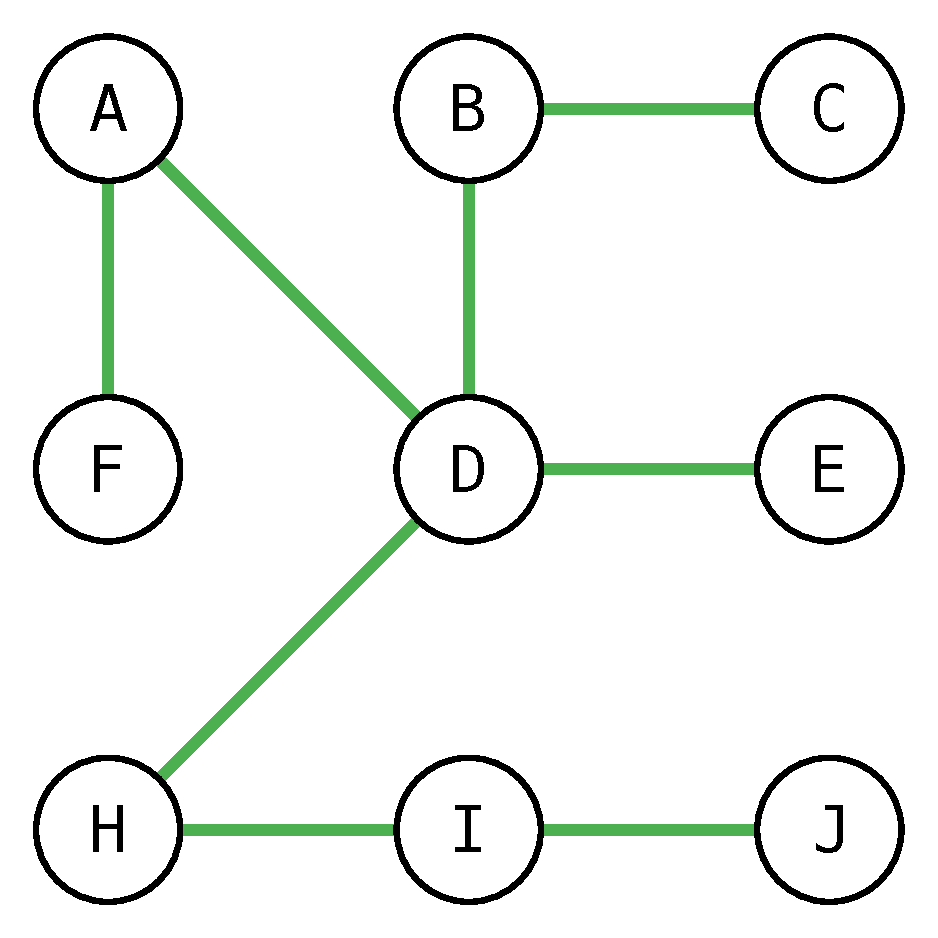
\includegraphics[width=0.42\textwidth]{figures/p20-chords-tree.pdf}\\[2pt]{\scriptsize б) остовное дерево $T_G(V, \hat{E})$ отдельно}} \\
\end{tabular}\end{center}
\grcap{Главные циклы: граф с хордами и его остов}

$G(V, E)$:
$T_G(V, \hat{E})$,\quad $E \setminus \hat{E} = \{e_1, \ldots, e_s\}$ --- набор хорд.

Добавление к дереву любой хорды $e_i$ создаёт ровно один цикл:
$\forall\, 1 \leq i \leq s$:\; $T_G(V, \hat{E}) \cup \{e_i\}$ содержит
цикл $\mathcal{E}_i$ --- \textbf{главный} (хорда $e_i$ плюс единственная
цепь в дереве между её концами).

$\mathcal{E}_1, \ldots, \mathcal{E}_s$ --- набор из $s$ главных циклов.

\medskip
\noindent\textbf{Пример.} Остов
$\hat{E} = \{BC, AD, BD, AF, DH, HI, IJ, DE\}$ (зелёные рёбра на
рисунке), хорды
$E \setminus \hat{E} = \{AB, DJ, BE, FH, EJ, CE\}$ (красные), $s = 6$.
Для каждой хорды выписываем цепь в дереве между её концами и замыкаем:

\begin{enumerate}
  \item $e_1 = AB$: цепь в дереве $A$--$D$--$B$ $\;\Rightarrow\; \mathcal{E}_1 = ABDA$
  \item $e_2 = DJ$: цепь $D$--$H$--$I$--$J$ $\;\Rightarrow\; \mathcal{E}_2 = DHIJD$
  \item $e_3 = BE$: цепь $B$--$D$--$E$ $\;\Rightarrow\; \mathcal{E}_3 = DBED$
  \item $e_4 = FH$: цепь $F$--$A$--$D$--$H$ $\;\Rightarrow\; \mathcal{E}_4 = DAFHD$
  \item $e_5 = EJ$: цепь $E$--$D$--$H$--$I$--$J$ $\;\Rightarrow\; \mathcal{E}_5 = DHIJED$
  \item $e_6 = CE$: цепь $C$--$B$--$D$--$E$ $\;\Rightarrow\; \mathcal{E}_6 = CBDEC$
\end{enumerate}

% ============================================================
% ЦИКЛОВОЕ ПРОСТРАНСТВО
% ============================================================

\subsection*{Цикловое пространство}

\begin{defn}{Сумма циклов}{cycle-sum}
$G(V, E)$,\; $l_1, l_2$ --- 2 цикла (замкнутых пути) в графе.

$l_1 \oplus l_2 := (e \in l_1) \;\Delta\; (e \in l_2)$

\quad (симметрическая разность рёбер).
\end{defn}

$A \,\Delta\, B = (A \cup B) \setminus (B \cap A) = 
\{a \in A \;\&\; a \notin B\} \cup \{a \notin A \;\&\; a \in B\}$:
общие рёбра <<сокращаются>>, остальные остаются.

\medskip
\noindent\textbf{Пример 1.} $\mathcal{E}_1 = ABDA$ (рёбра $AB, BD, DA$),
$\mathcal{E}_6 = CBDEC$ (рёбра $CB, BD, DE, EC$). Общее ребро $BD$
сокращается:
\[
  \mathcal{E}_1 \oplus \mathcal{E}_6
  = \{AB,\; DA,\; CB,\; DE,\; EC\}
  = ABCEDA
\]
--- снова цикл ($A$--$B$--$C$--$E$--$D$--$A$).

\medskip
\noindent\textbf{Пример 2.} $\mathcal{E}_5 = DHIJED$ (рёбра
$DH, HI, IJ, JE, ED$), $\mathcal{E}_4 = DAFHD$ (рёбра $DA, AF, FH, HD$).
Общее ребро $DH$ сокращается:
\[
  \mathcal{E}_5 \oplus \mathcal{E}_4
  = \{HI,\; IJ,\; JE,\; ED,\; DA,\; AF,\; FH\}
  = ADEJIHFA
\]
--- цикл $A$--$D$--$E$--$J$--$I$--$H$--$F$--$A$.

\medskip
\noindent\textbf{Пример 3.} Сложим все четыре:
\[
  l = \mathcal{E}_1 \oplus \mathcal{E}_6 \oplus \mathcal{E}_5 \oplus \mathcal{E}_4
  = (\mathcal{E}_1 \oplus \mathcal{E}_6) \oplus (\mathcal{E}_5 \oplus \mathcal{E}_4).
\]
У циклов $ABCEDA$ и $ADEJIHFA$ общие рёбра $AD$ и $DE$ сокращаются:
\[
  l = \{AB,\; BC,\; CE,\; EJ,\; JI,\; IH,\; HF,\; FA\} = ABCEJIHFA
\]
--- цикл по <<внешнему контуру>> графа, составленный из главных циклов
$\mathcal{E}_1, \mathcal{E}_6, \mathcal{E}_5, \mathcal{E}_4$.

\medskip
\textbf{Замечание.}
\begin{enumerate}[label=\alph*)]
  \item Множество всех <<обобщённых циклов>> (рёберно-непересекающихся
        объединений циклов, включая пустое множество рёбер) с операцией
        $\oplus$ образует векторное пространство над полем $\mathbb{F}_2$
        --- \textbf{цикловое пространство} графа;
  \item главные циклы $\mathcal{E}_1, \ldots, \mathcal{E}_s$ --- базис
        этого пространства: они линейно независимы (каждый содержит
        <<свою>> хорду, которой нет в остальных), и любой цикл $l$
        раскладывается по ним --- $l$ есть сумма главных циклов тех
        хорд, которые входят в $l$;
  \item размерность циклового пространства равна числу хорд:
        $s = |E| - |\hat E| = |E| - (|V| - 1) = |E| - |V| + 1$
        (\emph{цикломатическое число} графа). В примере выше:
        $s = 14 - 9 + 1 = 6$.
\end{enumerate}

\medskip
\textbf{Упр.} $G(V, E)$ --- связный, fix $T_G(V, \hat{E})$,
$\mathcal{E}_1, \ldots, \mathcal{E}_s$ --- главные циклы. Доказать
аккуратно пункты a) и b) замечания: что $(\{\text{обобщённые циклы}\},
\oplus)$ --- векторное пространство над $\mathbb{F}_2$ и что
$\mathcal{E}_1, \ldots, \mathcal{E}_s$ --- его базис.

% ============================================================
\begin{task}{Минимальное остовное дерево: алгоритм Краскала}{kruskal-task}
\textbf{Условие.} Дан неориентированный взвешенный граф на вершинах
$A,B,C,D,E,F,G$ с рёбрами
\begin{gather*}
  AB=7,\quad AD=5,\quad BC=8,\quad BD=9,\quad BE=7,\quad CE=5,\\
  DE=15,\quad DF=6,\quad EF=8,\quad EG=9,\quad FG=11.
\end{gather*}
Постройте минимальное остовное дерево алгоритмом Краскала. Укажите
порядок включения рёбер и суммарный вес.

\begin{center}
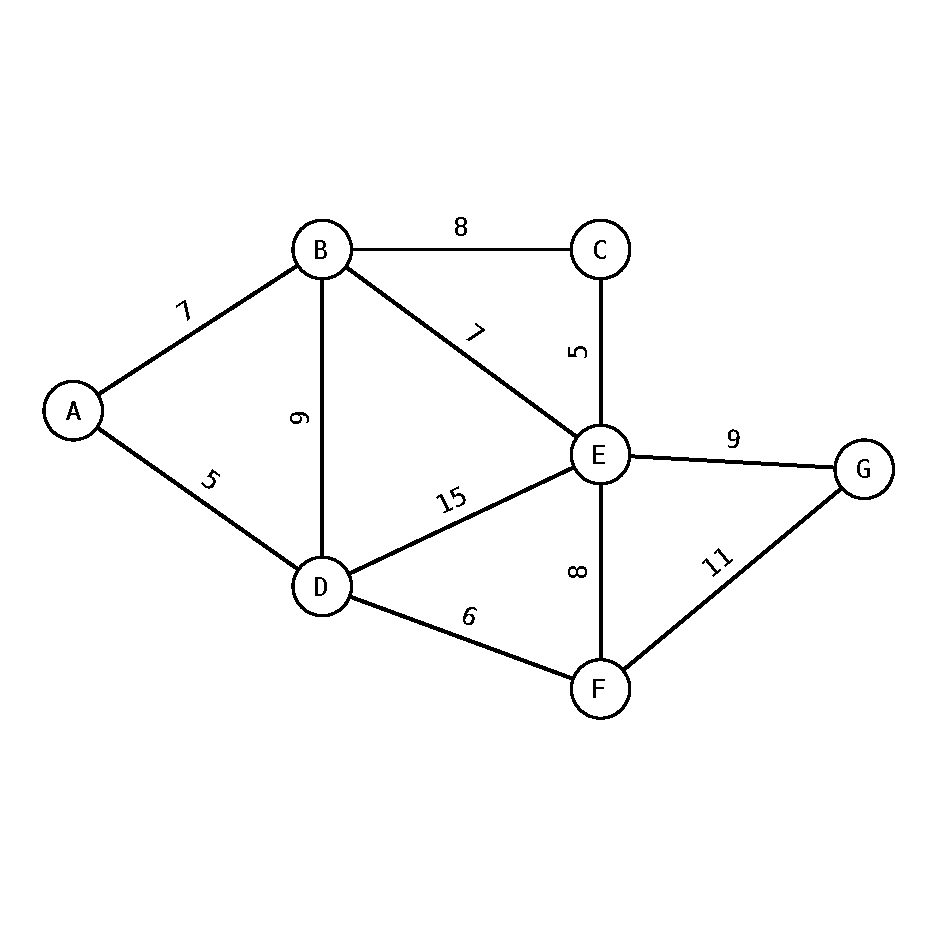
\includegraphics[width=0.5\textwidth]{figures/task-kruskal-1.pdf}
\end{center}

\textbf{Решение.} Краскал сортирует рёбра по возрастанию веса и добавляет ребро,
если его концы лежат в разных компонентах (что отслеживается системой
непересекающихся множеств) --- иначе ребро замкнуло бы цикл.

Отсортированный список рёбер:
\[
  AD(5),\ CE(5),\ DF(6),\ AB(7),\ BE(7),\ BC(8),\ EF(8),\ BD(9),\ EG(9),\ FG(11),\ DE(15).
\]
\begin{enumerate}
  \item $AD(5)$ --- компоненты $\{A\},\{D\}$ различны, добавляем $\Rightarrow\{A,D\}$.
  \item $CE(5)$ --- добавляем $\Rightarrow\{C,E\}$.
  \item $DF(6)$ --- $F$ присоединяется к $\{A,D\}$, добавляем $\Rightarrow\{A,D,F\}$.
  \item $AB(7)$ --- $B$ присоединяется, добавляем $\Rightarrow\{A,B,D,F\}$.
  \item $BE(7)$ --- сливаем $\{A,B,D,F\}$ и $\{C,E\}$, добавляем
        $\Rightarrow\{A,B,C,D,E,F\}$.
  \item $BC(8)$ --- $B$ и $C$ уже в одной компоненте: \emph{цикл, пропускаем}.
  \item $EF(8)$ --- цикл, пропускаем.
  \item $BD(9)$ --- цикл, пропускаем.
  \item $EG(9)$ --- $G$ присоединяется, добавляем. Все $7$ вершин в одной
        компоненте, набрано $6 = 7 - 1$ рёбер --- остов построен.
  \item $FG(11),\ DE(15)$ --- цикл, пропускаем.
\end{enumerate}

\medskip
\noindent Ключевые шаги построения:

\begin{center}\begin{tabular}{ccc}
\shortstack{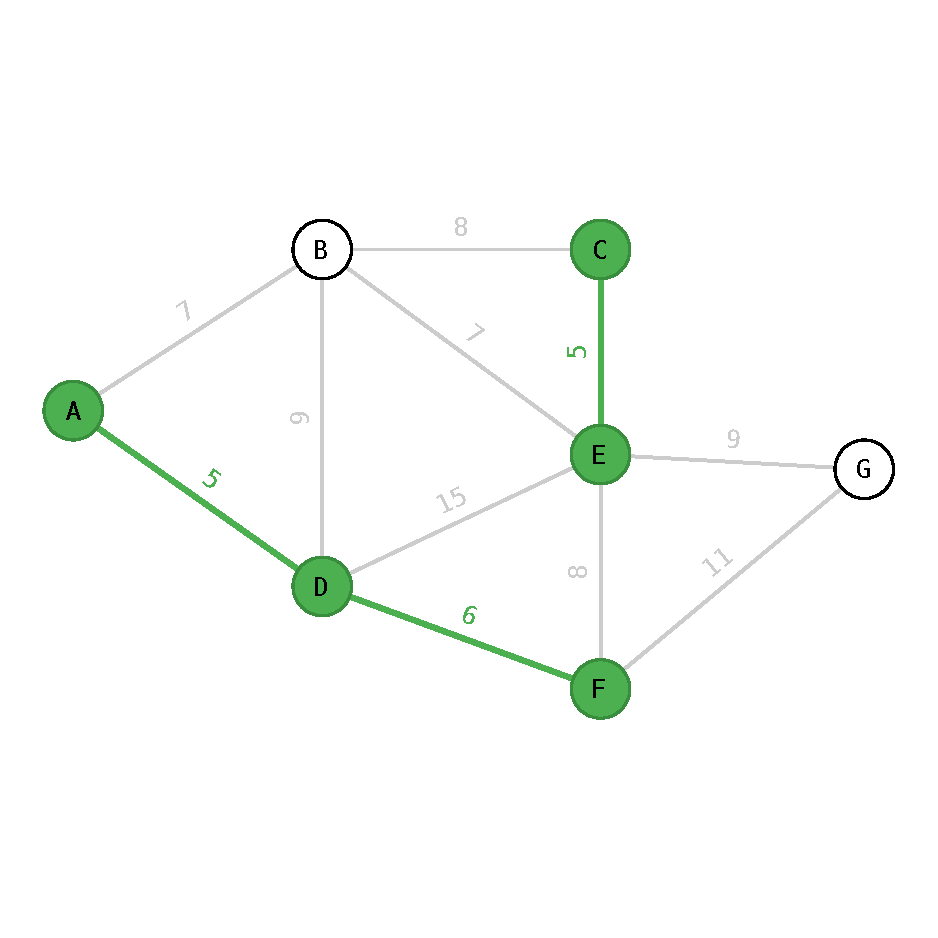
\includegraphics[width=0.30\textwidth]{python/lec08/kruskal_task/kruskalt-3.pdf}\\[2pt]{\scriptsize $+AD, +CE, +DF$}} &
\shortstack{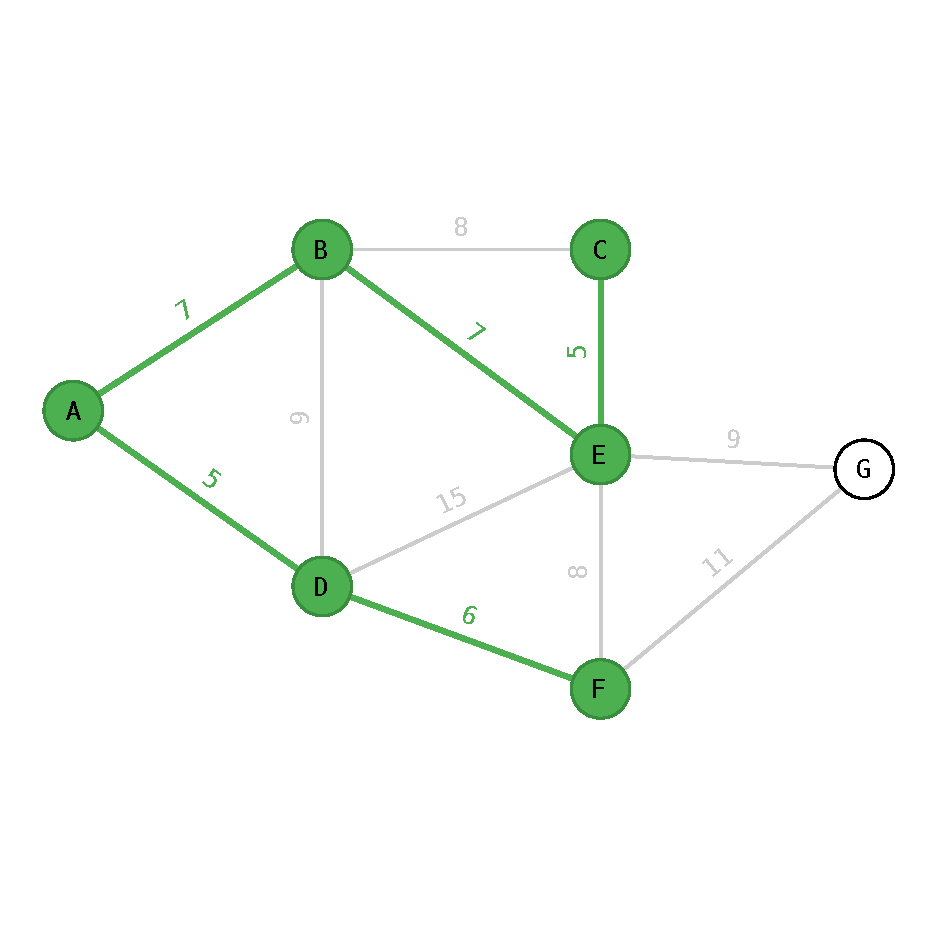
\includegraphics[width=0.30\textwidth]{python/lec08/kruskal_task/kruskalt-5.pdf}\\[2pt]{\scriptsize $+AB, +BE$}} &
\shortstack{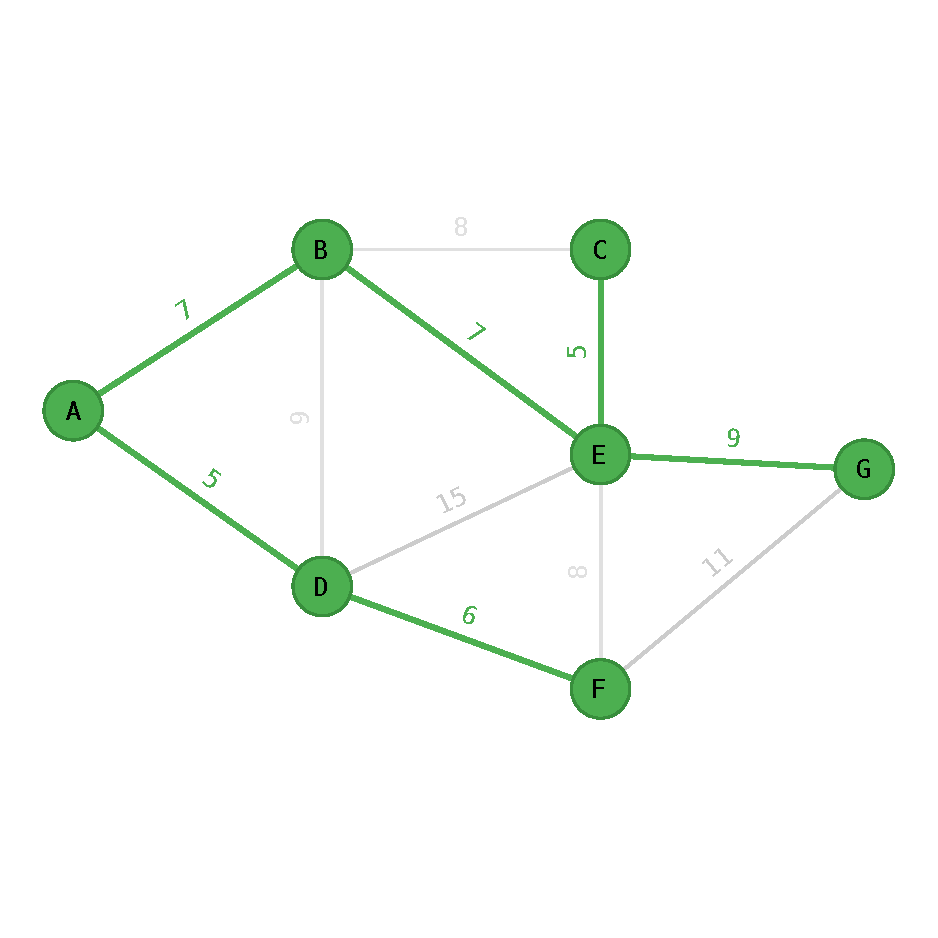
\includegraphics[width=0.30\textwidth]{python/lec08/kruskal_task/kruskalt-9.pdf}\\[2pt]{\scriptsize пропуски $BC, EF, BD$; $+EG$}} \\
\end{tabular}\end{center}
\begin{center}
\shortstack{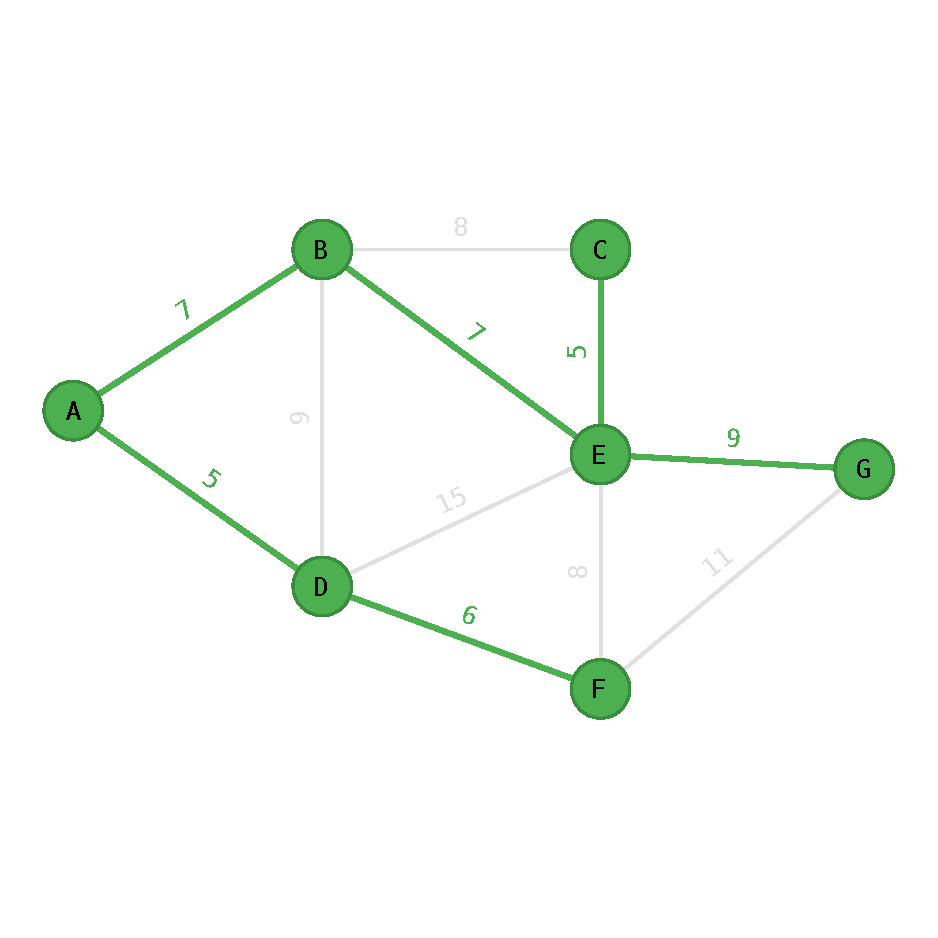
\includegraphics[width=0.34\textwidth]{python/lec08/kruskal_task/kruskalt-12.pdf}\\[2pt]{\scriptsize Остов построен, $\Sigma = 39$}}
\end{center}

\textbf{Ответ.} Остовное дерево: рёбра $AD,CE,DF,AB,BE,EG$; суммарный вес
$5+5+6+7+7+9=39$.
\end{task}
